\chapter{Methodology}
\label{ch:methodology}
\glsresetall

{
Heres what Im going to do right now:


1. Finish code to include:
  a. Ingest Measured object data
  b. Ingest sim'd object data
  c. Polar plots for both pols at 10GHz
    i. dashed lines to identify scattering centers
    ii. overlay plots over image
    iii. Overlay several rcs plots
    iv. plots of prob values?
  d. Frequency plots for both pols at
    i. 3D plot for freq slices f vs A vs azimuth
    ii. overlay sim and measurement?
  e. Extract probability metrics
    i. Amp, mean, var of each slice over frequency
2.

}

\section{Calibration}

Target measurements are unknown to the observer until they have been calibration. Range calibration is done by first subtracting background measurements from the target data. The corrected target data is then normalized using a ratio of simulated and measured truth data from the calibration object. The calibration object is a 7.5 inch cylinder. Additionally, background measurements are taken for both the calibration cylinder and target mounts. The formula for target calibration is shown in equation \ref{eq:cal} [CITE].

\begin{equation}\label{eq:cal}
    \sigma_{t, true} = \frac{\sigma_{t, raw} - \sigma_{t, bg}}{\sigma_{c, raw} - \sigma_{c, bg}}\sigma_{c, true}
\end{equation}

The raw and true measurements for the target and calibration cylinders are $\sigma_{t, raw}$, $\sigma_{t, true}$, $\sigma_{c, raw}$, and $\sigma_{c, true}$ respectively. The background measurements are taken of the target and calibration cylinders mounts, shown in the equation as $\sigma_{t, bg}$, $\sigma_{t, bg}$ respectively.

\section{RCS Calculation}

Target RCS is defined by the IEEE as shown in equation \ref{eq:ieee_rcs}\cite{Knott}.

\begin{equation}\label{eq:ieee_rcs}
    \sigma [m^2] = 4\pi \frac{|E_{r}|^2}{|E_{r}|^2}
\end{equation}

\section{Target Selection}
\label{sec:anothersectionRefName}

This experiment is concerned with identifying the capability of a machine learning algorithm to correctly classify real radar measurements. To examine this interaction directly, targets have been chosen that produce readily measurable radar responses in a compact range. Three targets have been chosen:  an oblate spheroid, a prolate spheroid, and a surrogate missile. The spheroid shapes were chosen due to their similarity, providing a classification stressor to the machine learning model. The surrogate missile has been chosen for three reasons:  the nose, tail, and sides of the missile will produce 3 distinct RCS responses; the intensity of the responses for the nose, tail, and sides will be large; it is critically important for a modern military to correctly identify an ingressing missile [CITE SOMETHING FROM UKRAINE...LINK TO WHAT AIR DEFENSE DOING LOL].

Each target is modeled in Blender 3D, and exported as a .stl file. The .stl file is then imported by FreeCAD, where it is convereted to a solid and exported as a .step file. Blender allows the easy development of complex mesh shapes that do not have "holes" or "seams". FreeCAD, while have more drafting tools, does not handle mesh creation well. Object files developed in FreeCAD and imported by CADFeko were rife with mesh errors, and Altair's CADFeko program does not handle mesh repair well. This development pipeline allowed for custom model development that could easily be imported to CADFeko.

CADFeko produces a final mesh overlay for the .step file. The size and dispersement of polygons in the final overlay are driven by the simulation frequency. "Discuss the sizing of polygons for electromagnetic simulations here, and cite something."

The physical dimensions, electrical length, and expected RCS response for each target will be detailed in the following sections.

\subsection{Prolate Spheroid}

The prolate sphere is oblong, measuring 6 inches along its longest axis, and 3 inches at its widest. The height and width of the prolate spheroid are equivalent.

\begin{figure}[htbp]
\centering
\begin{subfigure}{.5\textwidth}
  \centering
  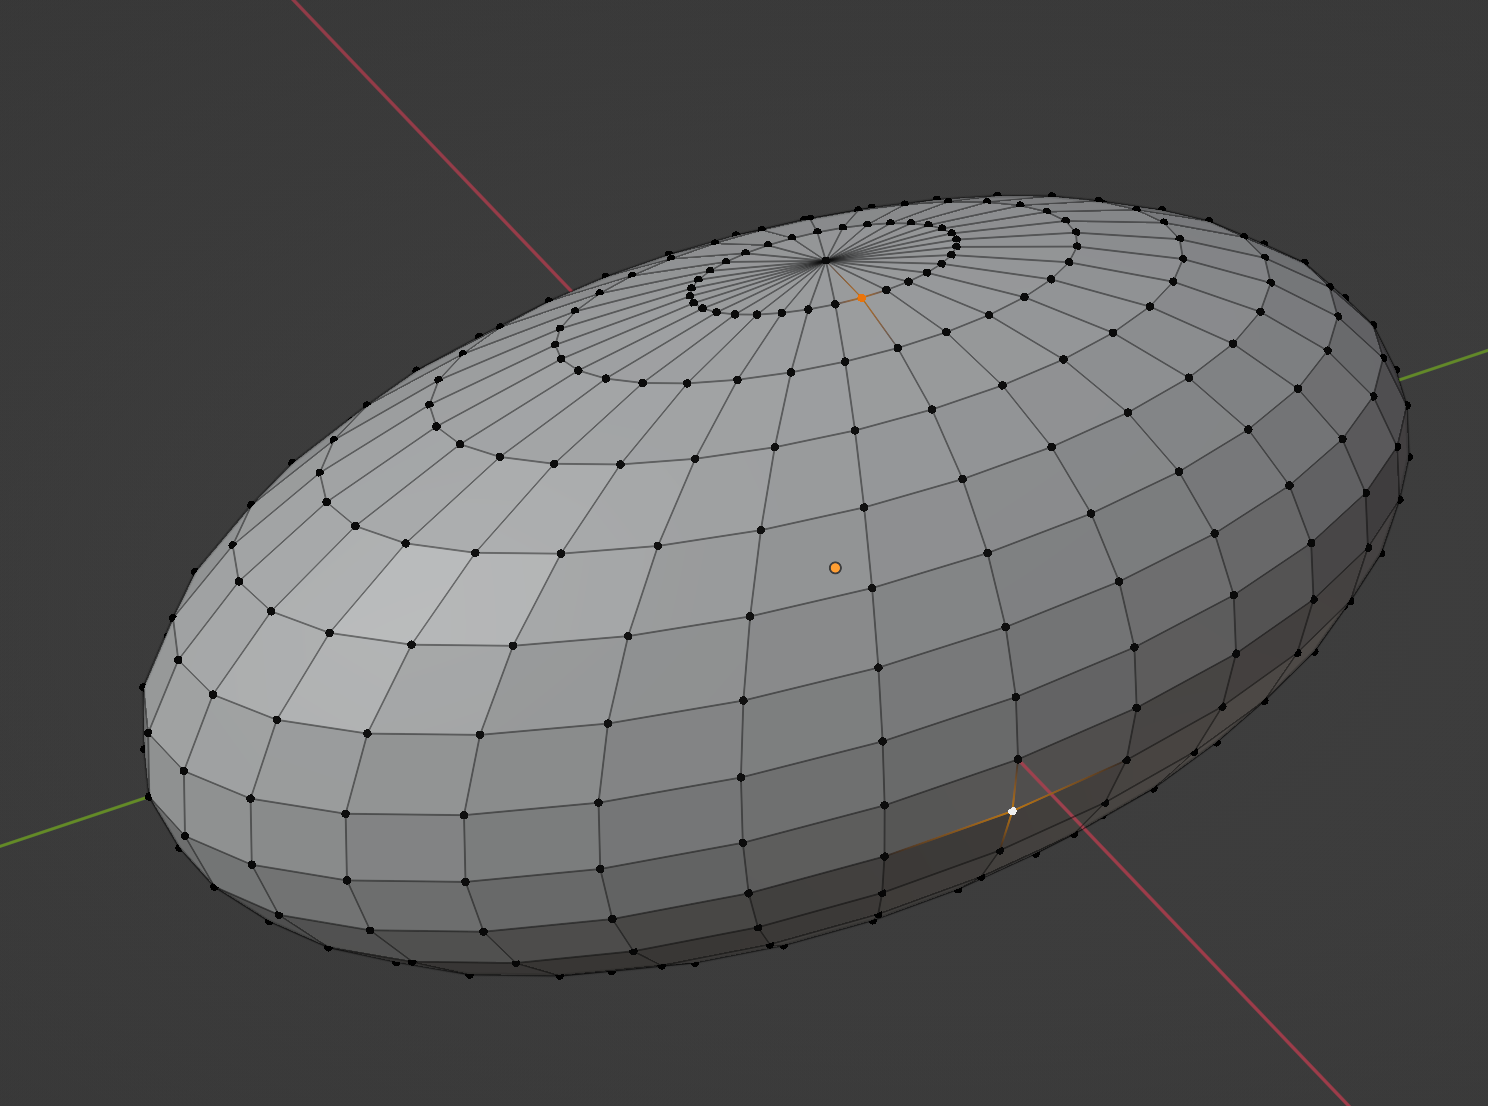
\includegraphics[width=.8\linewidth]{prolate_sphere_model.png}
  \caption{Prolate sphere modeled in Blender 3D.}
  \label{fig:ps_model}
\end{subfigure}%
\begin{subfigure}{.5\textwidth}
  \centering
  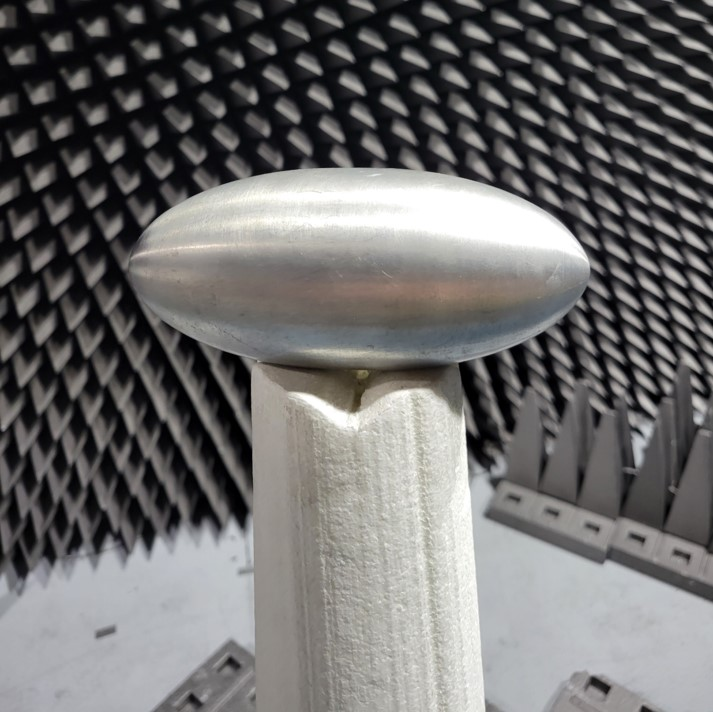
\includegraphics[width=.8\linewidth]{prolate_sphere_mounted.jpg}
  \caption{Mounted prolate sphere.}
  \label{fig:ps_mount}
\end{subfigure}
\caption{The simulated and physically mounted prolate sphere.}
\label{fig:ps}
\end{figure}

\subsection{Oblate Spheroid}

The oblate spheroid is rotationally symmteric, with a radius of 6 inches. The poles of the spheroid are 3 inches apart.

\begin{figure}[htbp]
\centering
\begin{subfigure}{.5\textwidth}
  \centering
  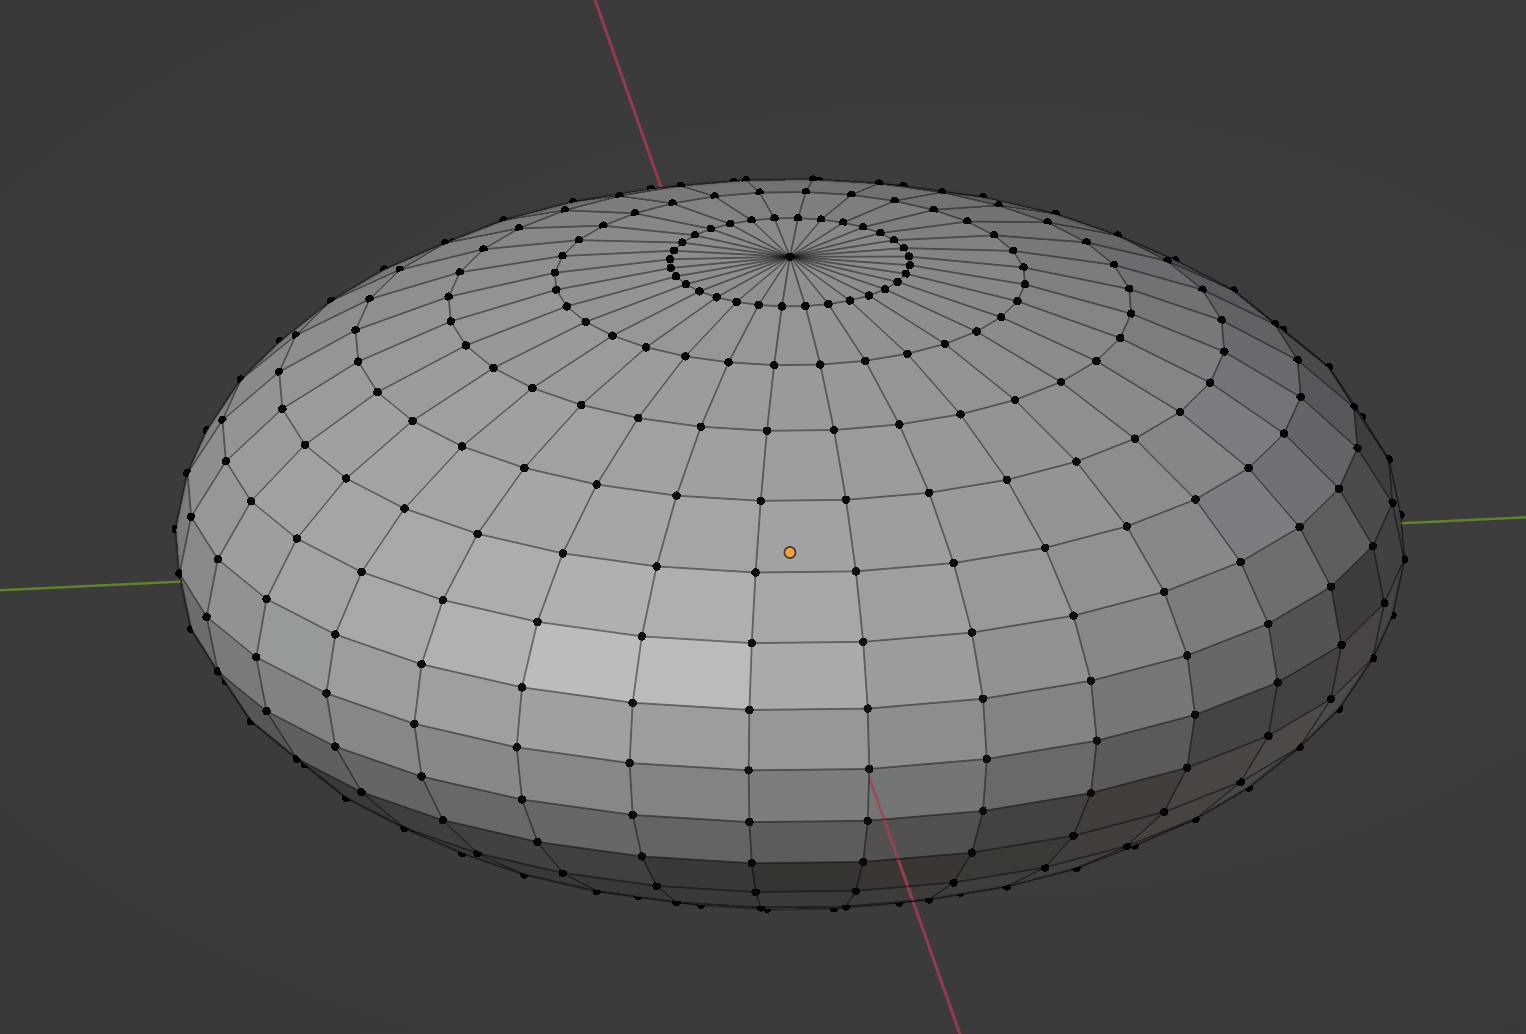
\includegraphics[width=.8\linewidth]{oblate_sphere_model.png}
  \caption{Oblate sphere modeled in Blender 3D.}
  \label{fig:os_model}
\end{subfigure}%
\begin{subfigure}{.5\textwidth}
  \centering
  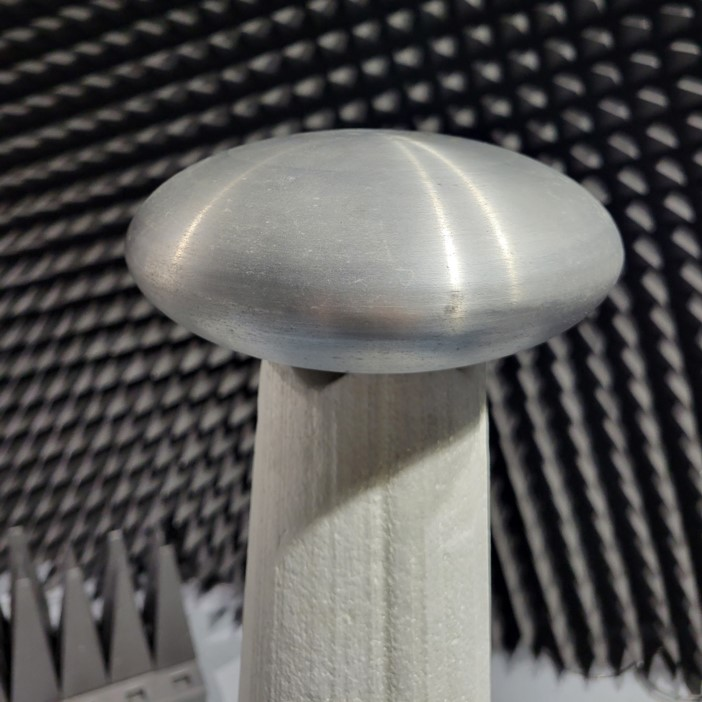
\includegraphics[width=.8\linewidth]{oblate_sphere_mounted.jpg}
  \caption{Mounted oblate sphere.}
  \label{fig:os_mount}
\end{subfigure}
\caption{The simulated and physically mounted oblate sphere.}
\label{fig:os}
\end{figure}

\subsection{Missile}
